\documentclass{VUMIFPSkursinis}
\usepackage{algorithmicx}
\usepackage{algorithm}
\usepackage{algpseudocode}
\usepackage{amsfonts}
\usepackage{amsmath}
\usepackage{bm}
\usepackage{caption}
\usepackage{color}
\usepackage{float}
\usepackage{graphicx}
\usepackage{listings}
\usepackage{subfig}
\usepackage{wrapfig}
\usepackage[backend=biber]{biblatex}

% Titulinio aprašas
\university{Vilniaus universitetas}
\faculty{Matematikos ir informatikos fakultetas}
\department{Programų sistemų katedra}
\papertype{Kursinis darbas}
\title{Didelių duomenų srautų analizė, anomalijų aptikimas}
\titleineng{Big data analysis, detection of anomalies}
\status{3 kurso 3 grupės studentas}
\author{Jokūbas Rusakevičius}
% \secondauthor{Vardonis Pavardonis}   % Pridėti antrą autorių
\supervisor{dr. Vytautas Valaitis}
\date{Vilnius – \the\year}

% Nustatymai
\setmainfont{Palemonas}   % Pakeisti teksto šriftą į Palemonas (turi būti įdiegtas sistemoje)
\bibliography{bibliografija}
%\addbibresource{bibliografija.bib}

\begin{document}
\maketitle

\tableofcontents

\sectionnonum{Įvadas}
%apie duomenis
Renkamų, saugomų ir operuojamų duomenų kiekiai nuolatos didėja ir gerokai lenkia žmogaus sugebėjimą juos apdoroti, peržiūrėti ar analizuoti. Didžiosios socialinių tinklų kompanijos Twitter, Facebook ir LinkedIn praneša kiekviena atskirai fiksuojanti iki 12 milijonų įvykių per sekundę \cite{twitter, facebook, linkedin}. Taip pat, vis daugiau duomenų yra surenkama iš automatizuotų duomenų šaltinių (pvz.: „Dalykų Interneto“ (angl. „Internet of Things“)). Kylantis automatizuotų duomenų šaltinių populiarumas, pinganti techninė įranga, išvystyti komunikaciniai tinklai bei mažėjančios duomenų saugojimo kainos paskatino dešimčių milijardų dolerių komercines investicijas šių technologijų vystimui \cite{iof_investments}. Numatoma, kad kiekvienais metais bendras duomenų kiekis išaugs po 40\% \cite{iof}. Tačiau žmogaus skiriamo dėmesio kiekis yra fiksuotas ir nekinta. Dėl šios priežasties, yra vis labiau neįmanoma remtis tik fizine šių „Didžiųjų Duomenų“ (angl „Big Data“) peržiūra. Taip pat, dėl didžiulio duomenų kiekio ir limituoto žmogaus dėmesio kiekio, dabartiniai aukščiausios klasės taikomųjų programų operatoriai praneša panaudojantys vos 6\% jų surenkamų duomenų \cite{prioritizing_attention}. \par
%apie fast data
Dabartinė „Didžiųjų Duomenų“ era su savimi atsinešė milžiniškus kiekius duomenų ir padėjo pagrindus naujai „Greitųjų Duomenų“ (angl. „Fast Data“) erai. „Greitųjų Duomenų“ era bus pažymėta didžiuliu duomenų pertekliumi ir resursų jų apdorojimui ir interpretavimui trūkumu \cite{prioritizing_attention}. Todėl atsiranda iššūkis, prioritizuoti dėmesį. Nors žmogui yra neįmanoma peržiūrėti visų šių duomenų, tačiau kompiuteriai ir mašinos gali. Informacinės sistemos labiau nei bet kada turi filtruoti, akcentuoti, jungti, grupuoti pateiktus duomenis ir rodyti naudotojui tik ribotą bei apibendrintą informaciją. Visa rodoma, bet nereikalinga informacija reikalauja ir eikvoja žmogaus dėmesį \cite{attention}. Tačiau, ypač dideli duomenų kiekiai gali būti per dideli ne tik žmogui, bet ir mašinai arba jos sugebėjimui ekonomiškai apdoroti duomenis dėl atliekamų skaičiavimų. Viso to pasekmė yra dažnas svarbaus funkcionalumo nepastebėjimas, dėl to krentantis efektyvumas bei atsakymų praradimas. \par
%apie macrobase
Stadfordo Universiteto ekspertai bei doktorantai, norėdami sugretinti žemo lygio duomenų srautų apdorojimo variklius su efektyviais ir tiksliais analitiniais varikliais gebančiais prioritizuoti dėmesį greituosiuose duomenyse, pradėjo kurti MacroBase \cite{macrobase_overview}, atviro kodo greitųjų duomenų analitinį variklį. MacroBase pagrindinis veikimo principas yra žmogaus dėmesio prioritizavimas. Šito uždavinio sprendimui naudojami analitiniai operatoriai, kurie identifikuoja reikšmingus taškus duomenų sraute, ir kurie sugretina, sulygina ir sugrupuoja panašumus tarp jų. Šie ir kiti operatoriai užtikrina, kad gražinamas rezultatas ir jo požymiai yra tikrai reikšmingi. Mažas pagrindinių greitųjų duomenų operatorių kiekis leidžia šiai sistemai likti lanksčiai ir lengvai pritaikomai įvairioms bei skirtingoms sistemoms. \par
%apie darbą TODO: FIX
Atviro kodo analitinis paieškos variklis MacroBase yra nuolatos kuriamas ir naujinamas. Šiuo darbu bus siekiama, įsidiegus šį variklį, ištirti MacroBase „Pašalinių“ (angl. „Outlier“) duomenyse aptikimo tikslumą naudojant skirtingus MacroBase algoritmus. Taip pat, priklausomai nuo gautų rezultatų pabandyti pagerinti tikslumą. Šiuo darbu tikimasi....


%Įvade apibūdinamas darbo tikslas, temos aktualumas ir siekiami rezultatai.
%Darbo įvadas neturi būti dėstymo santrauka. Įvado apimtis 1–2 puslapiai.


% \section{Medžiagos darbo tema dėstymo skyriai}
% Medžiagos darbo tema dėstymo skyriuose pateikiamos nagrinėjamos temos detalės:
% pradinė medžiaga, jos analizės ir apdorojimo metodai, sprendimų įgyvendinimas,
% gautų rezultatų apibendrinimas. Šios dalies turinys labai priklauso nuo darbo
% temos. Skyriai gali turėti poskyrius ir smulkesnes sudėtines dalis, kaip
% punktus ir papunkčius.

% Medžiaga turi būti dėstoma aiškiai, pateikiant argumentus. Tekstas dėstomas
% trečiuoju asmeniu, t.y. rašoma ne „aš manau“, bet „autorius mano“, „autoriaus
% nuomone“. Reikėtų vengti informacijos nesuteikiančių frazių, pvz., „...kaip jau
% buvo minėta...“, „...kaip visiems žinoma...“ ir pan., vengti grožinės literatūros
% ar publicistinio stiliaus, gausių metaforų ar panašių meninės išraiškos
% priemonių.

% \subsection{Poskyris}
% Citavimo pavyzdžiai: cituojamas vienas šaltinis \cite{PvzStraipsnLt}; cituojami
% keli šaltiniai \cite{PvzStraipsnEn, PvzKonfLt, PvzKonfEn, PvzKnygLt, PvzKnygEn,
% PvzElPubLt, PvzElPubEn, PvzMagistrLt, PvzPhdEn}.

\section{Greitųjų duomenų dėmesio prioritizavimas}
Greitųjų duomenų analizavimo sistemos privalo prioritizuoti programuotojų, kūrėjų, naudotojų ir mašinų dėmesį, akcentuodamos tik tikrai reikšmingus duomenis. Šiame skyriuje bus pristatyti trys kūrimo principai nepakankamo dėmesio prioritizavimui \cite{prioritizing_attention}, kuriais remiantis yra kuriamas MacroBase. Pirma, rodomi rezultato duomenys gali būti apibendrinti, sujungti ir kontekstualizuoti, taip sufokusuojant srities eksperto dėmesį \ref{subsec:rezultato}. Antra, iteracinio kūrimo palengvinimui, inžineriniai resursai turėtų būti protingai skirstomi į sąsajas (angl. „Interfaces“) \ref{subsec:iteracijų}. Trečia, arčiausiai duomenų šaltinio esantys skaičiavimo resursai gali būti skiriami tik didžiausią įtaką rezultatui turintiems duomenims \ref{subsec:skaičiavimų}.
 
\subsection{Rezultato prioritizavimas} \label{subsec:rezultato}
Žmogaus dėmesys yra fiksuotas, todėl vos keli per sekundę neapdorotų duomenų (angl. „Raw Data“) rezultatai parodyti sistemos naudotojui gali būti neįveikiamai daug. Priklausomai nuo sistemos masto, net sekundė skirta kiekvienam neapdorotų duomenų rezultatui stabdo darbo procesą. Be to, duomenų srautai fiksuojantys šimtus tūkstančių ar net daugiau įvykių per sekundę nebėra retas atvejis. Todėl su tokiais duomenų srautais dirbančios greitųjų duomenų sistemos negali sau leisti grąžinti ir rodyti sistemos naudotojui rezultatą su rodomais neapdorotais duomenimis.\par
Rezultato prioritizavimas yra pasiekiamas grąžinant daugiau informacijos su mažesne išeiga. Tai reiškia, kad rodoma naudotojui ne daug konkrečių rezultatų, o keli apibendrinti ir sugrupuoti. Be to, greituosius duomenis prioritizuodamos bei atlikdamos sprendimą, kokius ir/ar kokio tipo duomenis rodyti naudotojui, sistemos turi tai atlikti protingai. Kaip rašoma knygoje „Dieter Rams“, greitųjų duomenų sistema turėtų grąžinti mažiau, bet geresnius rezultatus  \cite{little_design}.\par
Pasiekti dėmesio prioritizavimo prioritizuojant rezultatą galima keliais būdais. Vienas iš būdų greitųjų duomenų sistemai tai padaryti yra apibendrinant ir apjungiant duomenis, taip suteikti jiems kontekstą ir akcentus pagrindiniams duomenų požymiams ar elgsenai duomenų junginio viduje ar duomenų visumoje. Pavyzdžiui, vietoje visų 200 tūkstančių probleminių įrašų gautų iš įrenginio 1225 grąžinimo ir atvaizdavimo, sistema galėtų grąžinti tik įrenginio identifikacinį kodą (šiuo atveju 1225) ir įtartinų įrašų skaičių (200 tūkst.). Dar vienas būda tolesniam dėmesio prioritizavimui gali būti rodymas duomenų pagal jų svarbumą ir reikšmingumą sistemos naudotojui. Taip pat, sistemos, duomenų junginiams ir duomenų svarumo reitingams paremti, gali pasinaudoti natūraliosiomis hierarchijomis ir ontologijomis, taip suteikdamos naudotojams galimybė gauti reikiamą informacijos detalumo lygi.

\subsection{Iteracijų prioritizavimas} \label{subsec:iteracijų}
Šiuolaikinė analizė ir jos darbo eiga susideda iš daug įvairių žingsnių, todėl pats svarbiausias aukštos kokybės analitinės sistemos projektavimo ir kūrimo principas yra iteracijos. Šie žingsniai apima: funkcijų kūrimą (angl. „Feature Engineering“), modelio pasirinkimą, parametrų reguliavimą ir efektyvumo inžineriją (angl. „Performance Engineering“). Be to, minėtieji žingsniai yra iš prigimties iteratyvūs ir varomi grįžtamuoju ryšiu (angl. „Feedback-driven“). Tačiau, didelė dalis ekspertų ekspertizių nėra paverčiamos analizėmis, nes modernios analizės darbo procesas reikalauja labai daug darbo jėgos. Yra skiriamos didelės lėšos, komandos ir daug aukštos kvalifikacijos mokslininkų, kurie dažnai atlieka vienodas, varginančias ir nuobodžias užduotis. Todėl, greitųjų duomenų sistemų užduotis turėtų būti: pasitelkusios išskirtinai iteracinį darbo procesą – pagreitinti grįžtamuoju ryšiu varomus procesus ir nuleisti reikalingų analizei atlikti žinių barjerą. \par
Sistemos projektavimo procesas turėtų suteikti sąlygas iteracijomis bei grįžtamuoju ryšių paremtam kūrimui. Yra geriau sistemai išlikti lanksčiai, nei tobulai tiksliai. Tai reiškia, kad yra geriau  suteikti sistemai naudingus numatytuosius nustatymus bei padaryti analizės darbo procesą lengvai konfigūruojama, nei užkrauti naudotojams naštą tai daryti patiems. Greitųjų duomenų sistemos iš naudotojų turėtų beveik nereikalauti jokio darbo, suteikdamos jiems lengvai naudojamus ir reguliuojamus analitinius įrankius. Turi būti vadovaujamasi mąstymu, kad pirmas modelis retai bus paskutinis, tam geri numatytieji nustatymai gali padėti gauti greitą grįžtamąjį ryšį bei rezultatus. Tačiau galingi sistemos įrankiai skirti patyrusiems ir aukštos kvalifikacijos sistemos naudotojams galintys konfigūruoti sudėtingąją analitinio darbo proceso pusę turėtų būt taip pat suteikiami. \par
Dauguma dabartinių sistemų gebančių atlikti tam tikrą užduotį gerai yra labai retai pritaikomos kitų užduočių sprendimui. Todėl, greitųjų duomenų sistema turėtų būt kuriama moduli ir iteratyviai plečiama. Sistemos naudotojai neturi atlikti vienodų, klaidoms atsirasti aplinkybes suteikiančių, nuobodžių ir varginančių užduočių, šios užduotys turėtų būti automatizuojamos sistemos, taip nuimant naštą nuo naudotojų. Visas naudotojo dėmesys turėtų būt sutelktas į taikomąją sritį ir į jai specifines žinias. Šie du principai suteikia net ir geriausiems analitiniams procesams galimybę didinti darbo mastą ir duomenų kiekį.

\subsection{Skaičiavimų prioritizavimas} \label{subsec:skaičiavimų}

\section{MacroBase duomenų analizės sistema}


\sectionnonum{Rezultatai ir išvados}
Rezultatų ir išvadų dalyje turi būti aiškiai išdėstomi pagrindiniai darbo
rezultatai (kažkas išanalizuota, kažkas sukurta, kažkas įdiegta) ir pateikiamos
išvados (daromi nagrinėtų problemų sprendimo metodų palyginimai, teikiamos
rekomendacijos, akcentuojamos naujovės).

\printbibliography[heading=bibintoc]
% Šaltinių sąraše nurodoma panaudota
% literatūra, kitokie šaltiniai. Abėcėlės tvarka išdėstomi darbe panaudotų
% (cituotų, perfrazuotų ar bent paminėtų) mokslo leidinių, kitokių publikacijų
% bibliografiniai aprašai.  Šaltinių sąrašas spausdinamas iš naujo puslapio.
% Aprašai pateikiami netransliteruoti. Šaltinių sąraše negali būti tokių
% šaltinių, kurie nebuvo paminėti tekste.

% \sectionnonum{Sąvokų apibrėžimai}
\sectionnonum{Santrumpos}
Sąvokų apibrėžimai ir santrumpų sąrašas sudaromas tada, kai darbo tekste
vartojami specialūs paaiškinimo reikalaujantys terminai ir rečiau sutinkamos
santrumpos.

\appendix  % Priedai
% Prieduose gali būti pateikiama pagalbinė, ypač darbo autoriaus savarankiškai
% parengta, medžiaga. Savarankiški priedai gali būti pateikiami ir
% kompaktiniame diske. Priedai taip pat numeruojami ir vadinami. Darbo tekstas
% su priedais susiejamas nuorodomis.

%\section{Niauroninio tinklo struktūra}
%\begin{figure}[H]
%    \centering
%    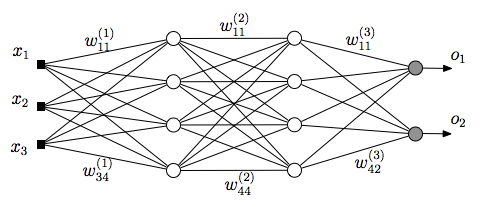
\includegraphics[scale=0.5]{img/MLP}
%    \caption{Paveikslėlio pavyzdys}
%    \label{img:mlp}
%\end{figure}
%
%
%\section{Eksperimentinio palyginimo rezultatai}
%% tablesgenerator.com - converts calculators (e.g. excel) tables to LaTeX
%\begin{table}[H]\footnotesize
%  \centering
%  \caption{Lentelės pavyzdys}
%  {\begin{tabular}{|l|c|c|} \hline
%    Algoritmas & $\bar{x}$ & $\sigma^{2}$ \\
%    \hline
%    Algoritmas A  & 1.6335    & 0.5584       \\
%    Algoritmas B  & 1.7395    & 0.5647       \\
%    \hline
%  \end{tabular}}
%  \label{tab:table example}
%\end{table}

\end{document}
